\documentclass{ximera}


\graphicspath{
  {./}
  {ximeraTutorial/}
  {basicPhilosophy/}
}

\newcommand{\mooculus}{\textsf{\textbf{MOOC}\textnormal{\textsf{ULUS}}}}

\usepackage{tkz-euclide}\usepackage{tikz}
\usepackage{tikz-cd}
\usetikzlibrary{arrows}
\tikzset{>=stealth,commutative diagrams/.cd,
  arrow style=tikz,diagrams={>=stealth}} %% cool arrow head
\tikzset{shorten <>/.style={ shorten >=#1, shorten <=#1 } } %% allows shorter vectors

\usetikzlibrary{backgrounds} %% for boxes around graphs
\usetikzlibrary{shapes,positioning}  %% Clouds and stars
\usetikzlibrary{matrix} %% for matrix
\usepgfplotslibrary{polar} %% for polar plots
\usepgfplotslibrary{fillbetween} %% to shade area between curves in TikZ
\usetkzobj{all}
\usepackage[makeroom]{cancel} %% for strike outs
%\usepackage{mathtools} %% for pretty underbrace % Breaks Ximera
%\usepackage{multicol}
\usepackage{pgffor} %% required for integral for loops



%% http://tex.stackexchange.com/questions/66490/drawing-a-tikz-arc-specifying-the-center
%% Draws beach ball
\tikzset{pics/carc/.style args={#1:#2:#3}{code={\draw[pic actions] (#1:#3) arc(#1:#2:#3);}}}



\usepackage{array}
\setlength{\extrarowheight}{+.1cm}
\newdimen\digitwidth
\settowidth\digitwidth{9}
\def\divrule#1#2{
\noalign{\moveright#1\digitwidth
\vbox{\hrule width#2\digitwidth}}}






\DeclareMathOperator{\arccot}{arccot}
\DeclareMathOperator{\arcsec}{arcsec}
\DeclareMathOperator{\arccsc}{arccsc}

















%%This is to help with formatting on future title pages.
\newenvironment{sectionOutcomes}{}{}


\author{Lee Wayand}

\begin{document}
\begin{exercise}  





Below is the graph of $y=f(t)$.  

\begin{image}
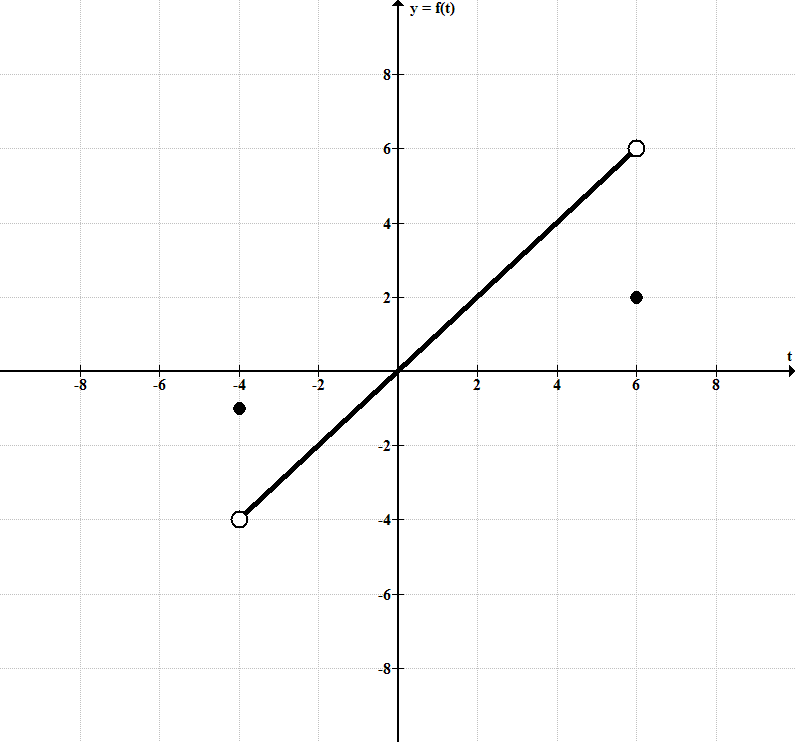
\includegraphics{../../pics/func_graphs/f32.png}
\end{image}


\begin{question} 

What is the domain of $f$?


\[
\left[ \answer[tolerance=0.25]{-4}, \answer[tolerance=0.25]{6} \right]
\]

\end{question}





\begin{question} 



Evaluate $f(-4) = \answer[tolerance=0.25]{-1}$


Classify $4$. \\


\begin{multipleChoice}
\choice [correct]{Discontinuity}
\choice {Singularity}
\choice {Neither}
\end{multipleChoice}




$-1$ is a local maximum of $f$ occuring at $-4$. \\


\begin{multipleChoice}
\choice [correct]{True}
\choice {False}
\end{multipleChoice}


\end{question}








\begin{question} 



Evaluate $f(6) = \answer[tolerance=0.25]{2}$


Classify $6$. \\


\begin{multipleChoice}
\choice [correct]{Discontinuity}
\choice {Singularity}
\choice {Neither}
\end{multipleChoice}




$2$ is a local minimum of $f$ occuring at $6$. \\


\begin{multipleChoice}
\choice [correct]{True}
\choice {False}
\end{multipleChoice}


\end{question}










\begin{question} 


$g$ is increasing on $(-4, 6)$. \\


\begin{multipleChoice}
\choice [correct]{True}
\choice {False}
\end{multipleChoice}




$g$ is increasing on $[-4, 6]$. \\


\begin{multipleChoice}
\choice {True}
\choice [correct]{False}
\end{multipleChoice}





$g$ is increasing on $[-4, 6)$. \\


\begin{multipleChoice}
\choice {True}
\choice [correct]{False}
\end{multipleChoice}




$g$ is increasing on $(-4, 6]$. \\


\begin{multipleChoice}
\choice {True}
\choice [correct]{False}
\end{multipleChoice}



\end{question}

















\begin{question} 

There exists a real number, $M$, such that $f(t) < M$ for all $t$.
\begin{multipleChoice}
\choice [correct]{True}
\choice {False}
\end{multipleChoice}





$f$ has a global maximum.
\begin{multipleChoice}
\choice {True}
\choice [correct]{False}
\end{multipleChoice}

\end{question}





\begin{question} 

There exists a real number, $M$, such that $f(t) > M$ for all $t$.
\begin{multipleChoice}
\choice [correct]{True}
\choice {False}
\end{multipleChoice}






$f$ has a global minimum.
\begin{multipleChoice}
\choice {True}
\choice [correct]{False}
\end{multipleChoice}





\end{question}










\begin{question} 


For every $\epsilon > 0$, the interval $(-4-\epsilon, -4+\epsilon)$ contains a domain number.
\begin{multipleChoice}
\choice [correct]{True}
\choice {False}
\end{multipleChoice}





For every $\epsilon > 0$, the interval $(-4-\epsilon, -4+\epsilon)$ contains a domain number, $d$, such that $f(d) - f(-4) > 1$.
\begin{multipleChoice}
\choice [correct]{True}
\choice {False}
\end{multipleChoice}


\end{question}














\begin{question} 


For every $\epsilon > 0$, the interval $(6-\epsilon, 6+\epsilon)$ contains a domain number.
\begin{multipleChoice}
\choice [correct]{True}
\choice {False}
\end{multipleChoice}





For every $\epsilon > 0$, the interval $(6-\epsilon, 6+\epsilon)$ contains a domain number, $d$, such that $f(d) - f(6) > 1$.
\begin{multipleChoice}
\choice [correct]{True}
\choice {False}
\end{multipleChoice}


\end{question}














\end{exercise}
\end{document}